\section{Gramática Livre de Contexto Probabilística}
\label{sec:pcfg}

Para descrever os modelos  probabilísticos  de \emph{parsing} de Michael Collins antes precisamos entender um pouco de Gramática Livre de Contexto Probabilística (PCFG - \emph{Probabilistic context-free grammar}).

PCFGs são uma extensão das gramáticas livres de contexto, só que existe uma probabilidade associada a cada regra de substituição.

Segundo Collins \cite{collins99}, o uso de técnicas estatísticas para o aprendizado de gramáticas foi inspirado no sucesso dessas técnicas para o processamento de fala. O modelo proposto em PCFG faz uma suposição de independência que considera a probabilidade de cada regra de substituição independente de todas as outras regras usadas na derivação da sentença. A ordem de derivação não afeta o modelo. As probabilidades atribuídas às regras nas PGFGs, são encaradas como a probabilidade do sintagma-pai usando tal regra, nos subelementos descritos, em comparação a todas as outras regras que expandem o mesmo sintagma.

Segundo Bonfante \cite{bonfante03}, as gramáticas probabilísticas têm muitas vantagens. Sendo elas extensões óbvias das gramáticas livres de contexto, os algoritmos usados para GLCs podem ser transportados para as PCFGs, permitindo que todas as possíveis análises possam ser encontradas num tempo de ordem $n^3$, em que n é o tamanho da sentença.

A ambiguidade é o maior problema na análise de sentenças. Uma gramática probabilística oferece solução para este problema, escolhendo a interpretação mais provável no momento da análise.

Vamos exemplificar: na frase ``vi o homem no monte com os binóculos", supondo a gramática parcial,

\begin{enumerate}
  \item $ S \rightarrow S \  SP^1 \ |\ SV $
  \item $ SV \rightarrow SV \ SP^2  \ |\  V \ SN \ |\ V \ SN \ SP^3 $
  \item $ SN \rightarrow SN \ SP^4  | \  N \  |  \ N \ SP^5 $
  \item $ SP \rightarrow P \ SN  $
\end{enumerate}

\begin{enumerate}
    \tiny
    \item SP modifica a sentença
    \item SP modifica o predicado
    \item SP é argumento (objeto indireto) do verbo
    \item SP modifica o sintagma nominal
    \item SP é complemento nominal
\end{enumerate}

Existe grande quantidade de árvores geradas, pois seria possível relacionar \emph{os binóculos} com \emph{no monte} com vários núcleos de sintagma como argumento ou modificador.

O caso anterior é genuinamente ambíguo (ambiguidade semântica), mas há muitos casos de ambiguidade que se devem apenas à gramática em si, ou seja, leitores percebem apenas uma interpretação.

Portanto, temos um problema quanto a descobrir qual a árvore de análise correta. Como solução poderíamos deixar que as situações de ambigüidade sejam resolvidas pela análise semântica, usar regras de desambiguação manuais ou usar modelos probabilísticos para atribuir probabilidades às diferentes árvores.

Uma gramática livre de contexto probabilística (PCFG) é uma quádrupla (N, T, $S_0$, R) onde:

 \begin{itemize}

   \item N: Conjunto de símbolos não-terminais
   \item T: Conjunto de símbolos terminais
   \item $S_0$: símbolo não-terminal, designado por símbolo inicial
   \item R: Conjunto de regras da forma $ A \rightarrow \alpha [p] $, onde:

    \begin{itemize}
      \item A é um símbolo não terminal;
      \item  $\alpha$ é uma cadeia de zero ou mais símbolos terminais e não terminais;
      \item p é um número entre 0 e 1 que representa a probabilidade condicional $P(\alpha | A)$ ( ou $P(A \rightarrow \alpha | A)$  ou de forma abreviada $P(A \rightarrow \alpha)$ ) de uma ocorrência de um dado não terminal em uma derivação ser expandida pela sequência $\alpha$.
    \end{itemize}

 \end{itemize}


$p=P(\alpha |A) = $ probabilidade de um dado não terminal A ser expandido na expressão $ \alpha. $

Sendo P uma função probabilística, a somatória das probabilidades sobre o universo de eventos deve resultar 1: 

$\sum_\alpha P(A \rightarrow \alpha)=1 $

Podemos usar uma PCFG para estimar a probabilidade associada a uma dada árvore, o que vai permitir arranjar uma solução para os casos de ambiguidade. 

Considerando a hipótese assumida pelas PCFG de que a probabilidade de expansão de cada constituinte é independente do contexto em que aparece na árvore global de análise, a probabilidade associada a cada árvore é o produto das probabilidades das regras usadas na sua derivação. Nas folhas da árvore, usam-se as probabilidades POS $P(\alpha_i|w_i)$, onde  $\alpha_i$ é a palavra e $w_i$ é a POS atribuída a palavra.

A estimativa das probabilidades associadas a cada regra pode ser feita usando um \emph{corpus} anotado de sentenças.

Supondo que haja n diferentes regras para expansão de A $A \rightarrow \alpha_i $, i de 1 a n.
\\
Pode-se então estimar $P(A \rightarrow \alpha_i|A)$ como:
\\

$ P(A \rightarrow \alpha_i) = \frac{count(A \rightarrow \alpha_i)}{\sum_{j=1}^n count(A \rightarrow \alpha_j)} = \frac{count(A \rightarrow \alpha_i)}{count(A)} $, onde count($A \rightarrow \alpha_i$) é o número de vezes que uma ocorrência de A é expandida pela regra $A \rightarrow \alpha_i$ no \emph{corpus} e count(A) é o número de vezes que uma ocorrência de A é expandida.

Consegue-se deste modo associar probabilidades às regras e construir uma gramática probabilística, por exemplo:

\begin{enumerate}
  \item  $SV \rightarrow Verbo [.50]$
  \item  $SV \rightarrow Verbo SN [.45]$
  \item  $SV \rightarrow Verbo SN SN [.05]$
\end{enumerate}

% Dado que uma árvore é constituída pelo conjunto de regras que participam na sua derivação.

\section{Trabalhos Anteriores, histórico de \emph{Parsing} Probabilístico para PLN}
\label{sec:trab_anter}

Segundo Manning e Sch{\"u}tze \cite{manning99}, o aprendizado estatístico se insere num contexto cuja linha de pesquisa é chamada de empírica, uma vez que se baseia em exemplos já prontos e aprende como lidar com aqueles ainda não vistos. A linha empiricista, que entre as décadas de 60 e 80 ficou nas sombras de crenças racionalistas encabeçadas por Chomsky (1965), cujo reflexo dentro da Inteligência Artificial caracterizava-se pela criação de sistemas inteligentes com grande quantidade de conhecimento inicial codificado à mão, ressurgiu na década de 90, com a idéia de que o conhecimento pode ser induzido a partir de algumas operações básicas de associação e generalização. Assim, segundo o empiricismo, uma máquina poderia aprender a estrutura de uma linguagem apenas observando uma grande quantidade de exemplos, usando procedimentos estatísticos gerais e métodos de associação e generalização indutiva, como aprendizado indutivo de regras.

Segundo Bonfante \cite{bonfante03}, o maior obstáculo encontrado pelos sistemas automáticos de \emph{parsing} (\emph{parsers}) surge quando estes se deparam com sentenças que possuem algum tipo de ambiguidade sintática, ou seja, sentenças com duas ou mais árvores possíveis. Por exemplo, na sentença ``A menina viu o menino de binóculo", a atribuição dos \emph{TAGS} sintáticos pode mudar a interpretação que se faz da frase. Duas árvores de representação são possíveis para a mesma sentença, nas quais, de acordo com a estrutura da primeira, a menina é que estava de binóculo e observou o menino, e na segunda, a menina observou o menino que estava de binóculo conforme ilustrado na Figura \ref{ambiguidade}. Nesses casos, é necessário que o \emph{parser} opte por uma delas, e que, de preferência, seja a que se esteja buscando.

\begin{figure}
	\begin{center}
		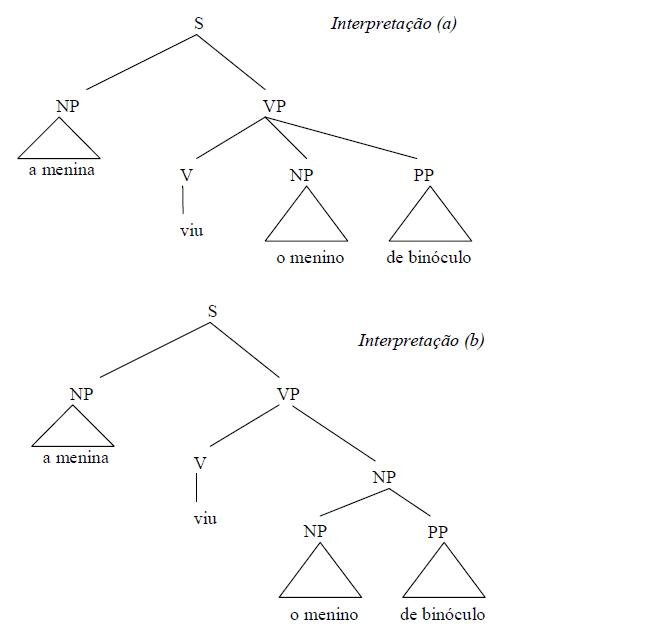
\includegraphics[scale=0.5]{ambig.jpg}
		\caption{\label{ambiguidade} Imagem das árvores da frase \emph{A menina viu o menino de binóculo}}		
	\end{center}
\end{figure}

Assim, segundo Bonfante \cite{bonfante03}, para que o \emph{parser} pudesse fazer a atribuição procurada, ele precisaria de uma certa interpretação de significado que o ajudasse a fazer a escolha correta. No entanto, tais sistemas são totalmente desprovidos de quaisquer informações nesse sentido. Muitos acham que essa não é uma função do \emph{parser}, delegando tal responsabilidade a uma unidade especial de desambiguação. Os \emph{parsers} estatísticos utilizam medidas de probabilidades observadas em sentenças previamente analisadas como critério de desempate em prováveis ações de desambiguação. Portanto, para que funcione, é necessário que se tenha um conjunto bastante representativo de sentenças com suas respectivas árvores sintáticas. Desse modo, o \emph{parser} atribuirá probabilidades às possíveis análises de uma sentença, apresentando como resposta aquela de maior probabilidade, sendo isso feito em três passos: (1) encontra todas as possíveis análises; (2) atribui-lhes probabilidades, e (3) seleciona a de mais alta probabilidade.


Um importante fator influenciador nas pesquisas no campo de PLN foi a disponibilização de grandes \emph{corpora} (\emph{treebanks}) anotados usados para treino dos analisadores probabilísticos.

\section{Problemas encontrados  na Gramática Livre de Contexto Probabilística}
\label{sec:prob_encontrados}

Segundo Bonfante \cite{bonfante03}, PCFGs foi o ponto de início natural para as pesquisas em desenvolvimento de \emph{parsers} estatísticos para PLN. Suas propriedades formais foram bem compreendidas, algoritmos eficientes para \emph{parsing} eram bem conhecidos e descritos. Mas após algumas  pesquisas descobriu-se que o uso apenas de PCFGs era insuficiente para PLN, e percepção de algumas deficiências na utilização de PCFGs em PLN gerou estudos profundos em três áreas na tentativa se achar métodos apropriados e eficientes para PLN estatística.

\begin{enumerate}
  \item Desenvolvimento de modelos mais sensíveis quanto as estruturas de linguagem.
  \item Desenvolvimento de modelos contendo parâmetros correspondentes às dependências léxicas.
  \item Desenvolvimento dos chamados ``\emph{history-based models}'' ou modelos baseados em históricos.
\end{enumerate}

\section{Métodos Probabilísticos com aumento de sensibilidade estrutural ou ao contexto}
\label{sec:aumento_sensibilidade}

Segundo Collins \cite{collins99}, muitas pesquisas foram voltadas ao objetivo de aumentar a sensibilidade ao contexto em uma PCFG, tendo resultados encorajadores. Considerando um modelo baseado em regras, mais uma vez, com mais sensibilidade ao contexto que PCFG. 

\section{Formalismo incluindo dependência lexical}
\label{sec:dependencia_lexical}

Segundo Collins \cite{collins99}, existem pelo menos duas razões para o desenvolvimento de modelos que incluem dependência de parâmetros. Primeiro, pesquisas interessadas em modelagem para reconhecimento da fala imaginavam que enquanto modelos ``\emph{trigram}'' teriam modelos sintáticos pobres, as probabilidades associadas aos pares ou triplas de palavras era muito úteis quando tinham probabilidades associadas às sentenças na linguagem. Segundo, o mais importante apontado por Michael Collins para seus estudos, pesquisas sugeriram que a dependência de probabilidade seria poderosa para abordar o problema da ambigüidade.

\section{Modelos de Michael Collins}
\label{sec:modelos_collins}

%``''

\begin{quotation}
\footnotesize
``Segundo Bonfante (\cite{bonfante03}, p. 45), Michael Collins propõe um modelo baseado em dependências lexicais entre bigramas. Este modelo usa informações lexicais para modelar relações núcleo-modificador. Também introduz um conceito de distância nesse modelo baseado em dependências entre bigramas. Segundo ele, a distância é uma variável crucial quando se decide se duas palavras estão relacionadas.

Após isso, Collins \cite{collins97} propõe três novos modelos gerativos de \emph{parsing}, que usam uma nova abordagem para melhorar o modelo de bigramas, todos eles baseados na noção \emph{head-centering}, em que o núcleo é o elemento principal e direcionador de todo o processo de geração de uma árvore sintática.

Collins define uma probabilidade conjunta P(AS; S) sobre pares árvore-sentença. Ele usa um modelo baseado no histórico de análise: uma árvore sintática é representada como uma seqüência de decisões, a partir de uma derivação \emph{top-down} e centrada no núcleo da árvore sintática. Segundo o autor, a representação da árvore sintática dessa forma permite que suposições de independência sejam feitas, levando a parâmetros condicionados a núcleos lexicais: parâmetros de projeção do núcleo, subcategorização, colocação de complemento/adjunto, dependência, distância, entre outros parâmetros.

A seguir é apresentado cada um dos modelos. O Modelo 2 representa uma evolução em relação ao Modelo 1; e o Modelo 3, em relação ao Modelo 2.''
\end{quotation}

\subsection{Modelo 1}
\label{sub:modelo1}

%``''

\begin{quotation}
\footnotesize
``Segundo Bonfante (\cite{bonfante03}, p. 53), este modelo apresenta uma proposta de como estender uma Gramática Livre de Contexto Probabilística (PCFG) para uma gramática lexicalizada (que considera itens lexicais). O Modelo 1 tem ainda parâmetros que correspondem a dependências entre pares de núcleos; a distância também é incorporada como uma medida, generalizando o modelo para uma abordagem baseada na história da análise.

A geração do lado direito da regra é quebrada em uma seqüência de pequenos passos. Cada regra passa a ter a forma:

$$Pai(nuc) = E_n(pe_n)...E_1(pe_1)NUC(nuc)D_1(pd_1)...D_m(pd_m)$$

Onde $NUC(nuc)$ representa o núcleo do sintagma, que recebe o item lexical nuc de seu pai $Pai$; $E_1...E_n e D_1...D_m$ são seus sintagmas modificadores, à esquerda e à direita de dentro do núcleo para as extremidades, com itens lexicais $pe$ e $pd$, respectivamente. As seqüências à direita e à esquerda são aumentadas com um símbolo STOP, de forma que permita um processo de Markov para o modelo. Assim, $ E_{n+1} = D_{m+1} = STOP $.

A regra de probabilidade pode ser reescrita usando a regra da cadeia de probabilidades:

$$P(E_{n+1}(pe_{n+1})...E_1(pe_1)NUC(nuc)D_1(pd_1)...D_{m+1}(pd_{m+1})|Pai(nuc)) = $$

$$P_{nuc}(NUC|Pai(nuc)) \times $$
$$\prod_{i=1..n+1} P_{esq}(E_i(pe_i)|E_1(pe_1)...E_{i-1}(pe_{i-1}), Pai(nuc),NUC) \times $$
$$\prod_{i=1..m+1} P_{dir}(D_j(pd_j)|E_1(pe_1)...E_{n+1}(pe_{n+1}),D_1(pd_1)...D_{j-1}(pd_{j-1}), Pai(nuc),NUC)  $$

Nota-se que a ordem de decomposição é: primeiro núcleo do sintagma, depois os modificadores de dentro para fora (núcleo para extremidades), sendo primeiro os modificadores a esquerda e depois os a direita.

Para um modelo ser Modelo Baseado na História da Análise ( MBHA), cada modificador poderia depender de qualquer função $\Theta$ dos modificadores anteriores, categoria do núcleo/pai e núcleo.

$$P_{esq}(E_i(pe_i)|E_1(pe_1)...E_{i-1}(pe_{i-1}), Pai(nuc),NUC) = $$
$$P_{esq}(E_i(pe_i)|\Theta(E_1(pe_1)...E_{i-1}(pe_{i-1}), Pai(nuc),NUC))$$

$$P_{dir}(D_j(pd_j)|E_1(pe_1)...E_{n+1}(pe_{n+1}),D_1(pd_1)...D_{j-1}(pd_{j-1}), Pai(nuc),NUC) = $$
$$P_{dir}(D_j(pd_j)|\Theta(E_1(pe_1)...E_{n+1}(pe_{n+1}),D_1(pd_1)...D_{j-1}(pd_{j-1}), Pai(nuc),NUC))$$

Fazendo a suposição de independência de que os modificadores são gerados independentemente uns dos outros, ou seja, fazendo $\Theta$ ignorar tudo a não ser P, NUC e nuc, temos

$$P_{esq}(E_i(pe_i)|E_1(pe_1)...E_{i-1}(pe_{i-1}), Pai(nuc),NUC) = P_{esq}(E_i(pe_i)|Pai(nuc),NUC)$$
$$P_{dir}(D_j(pd_j)|E_1(pe_1)...E_{n+1}(pe_{n+1}),D_1(pd_1)...D_{j-1}(pd_{j-1}), Pai(nuc),NUC) =$$
$$P_{dir}(D_j(pd_j)|Pai(nuc),NUC)$$

A geração de um lado direito de um regra, dado o lado esquerdo, é então feita em
três passos, sucessivamente, até que toda a árvore seja construída: (1) gera-se o núcleo (NUC); (2) geram-se modificadores à esquerda (E) e (3) geram-se modificadores à direita (D).''
\end{quotation}

\subsubsection{Adicionando Distância}
\label{sub:distancia}

\begin{quotation}
\footnotesize
``Segundo Bonfante (\cite{bonfante03}, p. 55), Michael Collins também adiciona distância a esse modelo. Essa adição é importante para capturar preferências relacionadas a modificação à direita (por exemplo, \emph{right pp attachment}) por estruturas de ligação à direita (que quase sempre traduz a preferência por dependências entre palavras adjacentes) e a preferência por dependências que não cruzam um verbo. A distância pode ser incorporada adicionando uma quantidade de dependência entre os modificadores.

$$P_{esq}(E_i(pe_i)|Pai,NUC, nuc,E_1(pe_1)...E_{i-1}(pe_{i - 1}) = $$
$$P_{esq}(E_i(pe_i)|NUC, Pai, nuc, distancia_{esq}(i - 1))$$
\\
$$P_{dir}(D_i(pd_i)|Pai,NUC, nuc,D_1(pd_1)...D_{i-1}(pd_{i - 1}) = $$
$$P_{dir}(D_i(pd_i)-NUC, Pai, nuc, distancia_{dir}(i - 1))$$
\\

A distância é um vetor contendo duas informações: adjacência (que permite aprender preferências associadas a modificadores à direita) e existência de um verbo entre eles (que permite aprender a preferência pela modificação do verbo mais recente).''
\end{quotation}

\subsection{Modelo 2}
\label{sub:modelo2}

\begin{quotation}
\footnotesize
``Segundo Bonfante (\cite{bonfante03}, p. 56), este modelo proposto por Collins, introduz a distinção entre complemento/adjunto. Os complementos  são acrescidos do sufixo ``C''. Assim, o modelo é estendido para fazer essa distinção e também para ter parâmetros que correspondam diretamente a distribuições de probabilidade sobre subcategorizações para núcleos.
O processo gerativo passa então a incluir escolha probabilística de subcategorização à esquerda ou à direita:

\begin{enumerate}
  \item Escolhe o núcleo com probabilidade $P_{nuc}(NUC|Pai, nuc)$
  \item Escolhe subcategorizações à esquerda e à direita, E-C e D-C, com probabilidades $P_{esq}(E-C|Pai,NUC, nuc)$ e $P_{dir}(D-C|Pai,NUC, nuc)$. Cada subcategorização é um conjunto que especifica os complementos que o núcleo requer como modificadores à direita ou à esquerda.
  \item Gera modificadores à esquerda e à direita com probabilidades

$P_{esq}(E_i(pe_i)|NUC, Pai, nuc, distancia_{esq}(i - 1),E - C)$ e

$P_{dir}(D_i(pd_i)|NUC, Pai, nuc, distancia_{dir}(i - 1),D - C)$

\end{enumerate}

Conforme os complementos são gerados, eles são removidos do conjunto de subcategorização (SUBCAT) apropriado. A probabilidade de gerar o símbolo STOP é 1 quando SUBCAT estiver vazio, e a probabilidade de gerar um complemento será 0 quando ela não estiver no SUBCAT.''
\end{quotation}

\subsection{Modelo 3}
\label{sub:modelo3}

\begin{quotation}
\footnotesize
``Segundo Bonfante (\cite{bonfante03}, p. 57), o modelo 3 é estendido da gramática de estrutura de frase generalizada para possibilitar tratamento de \emph{Wh-movement}\footnote{A modificação do modelo 3 não se mostra relevante e não é contemplada no \emph{parser} do Bikel, nem neste trabalho.}. Introduz parâmetros TRACES e Wh-Movement. Por exemplo, na frase ``\emph{The store that IBM bought last week}", o modelo usaria as regras para gerá-la:

\begin{enumerate}
  \item $SN \rightarrow SN SBAR(+gap)$
  \item $SBAR(+gap) \rightarrow Wh_{sn} S-C(+gap)$
  \item $S(+gap) \rightarrow SN-C SV(+gap)$
  \item $SV(+gap) \rightarrow Verbo Trace SN$
\end{enumerate}


SBAR é a representação para subcláusula; gap é a indicação de que falta algo naquele espaço.''
\end{quotation}

%\section{Casos especiais}
%\label{sec:modelo3_casos_especiais}

%Há regras especiais para derivação de coordenação e geração de símbolos de pontuação.
